\chapter{Аналитический раздел}
\label{cha:analysis}

В данном разделе приводится понятие ситуации гонки, рассматривается классификация существующих методов поиска гонок в программах, выявляются достоинства и недостатки каждого из методов. Раздел содержит описание существующих методов статического поиска гонок в программах, описание основных идей, лежащих в их основе, рассматриваются современные проблемы статического поиска гонок.

\section{Понятие ситуации гонки}

Под состоянием гонки при множественном доступе к разделяемой памяти будем понимать ситуацию, когда два или более потоков одновременно совершают доступ к разделяемой области памяти, и, по крайней мере, хотя бы один из них выполняет операцию записи в неё.

В листинге~\ref{lst:race} показан пример программы, в которой возможно возникновение гонок при доступе к разделяемой переменной $count$. Доступ к ней в функции $foo$ является не защищенным ни одним из средств взаимоисключения. Это может привести к возникновению гонок при одновременном доступе к ней из различных потоков. В листинге~\ref{lst:protected} показан пример исправленной программы из листинга~\ref{lst:race}. Гонки при доступе к разделяемой переменной $count$ в нём устраняются посредством использования средства синхронизации — мьютекса $lock$.

\lstinputlisting[language=C,caption=Пример возникновения гонки при доступе к разделяемой переменной (\Code{race.c}),label=lst:race]{inc/src/race.c}

\lstinputlisting[language=C,caption=Пример защмщенного доступа к разделяемой переменной (\Code{protected.c}),label=lst:protected]{inc/src/protected.c}

\section{Граф потока управления}

Одним из основных способов представления потока выполнения программы является граф потока управления - ориентированный граф, отражающий множество всех возможных путей исполнения, в котором, как правило, выделяют две специальные вершины start (вершина начала) и stop (вершина конца), такие, что в start не заходит ни одна дуга, из stop не выходит ни одна дуга.

В графе потока управления каждый узел (вершина) графа соответствует базовому блоку - прямолинейному участку кода, не содержащего в себе ни операций передачи управления, ни точек, на которое управление передается из других частей программы. В качестве примера на рис.~\ref{fig:cfg-example} представлен граф потока
управления для программы, представленной в листинге~\ref{lst:cfg}.

\lstinputlisting[language=C,caption=Пример программы (\Code{cfg.c}),label=lst:cfg]{inc/src/cfg.c}

\begin{figure}
  \centering
  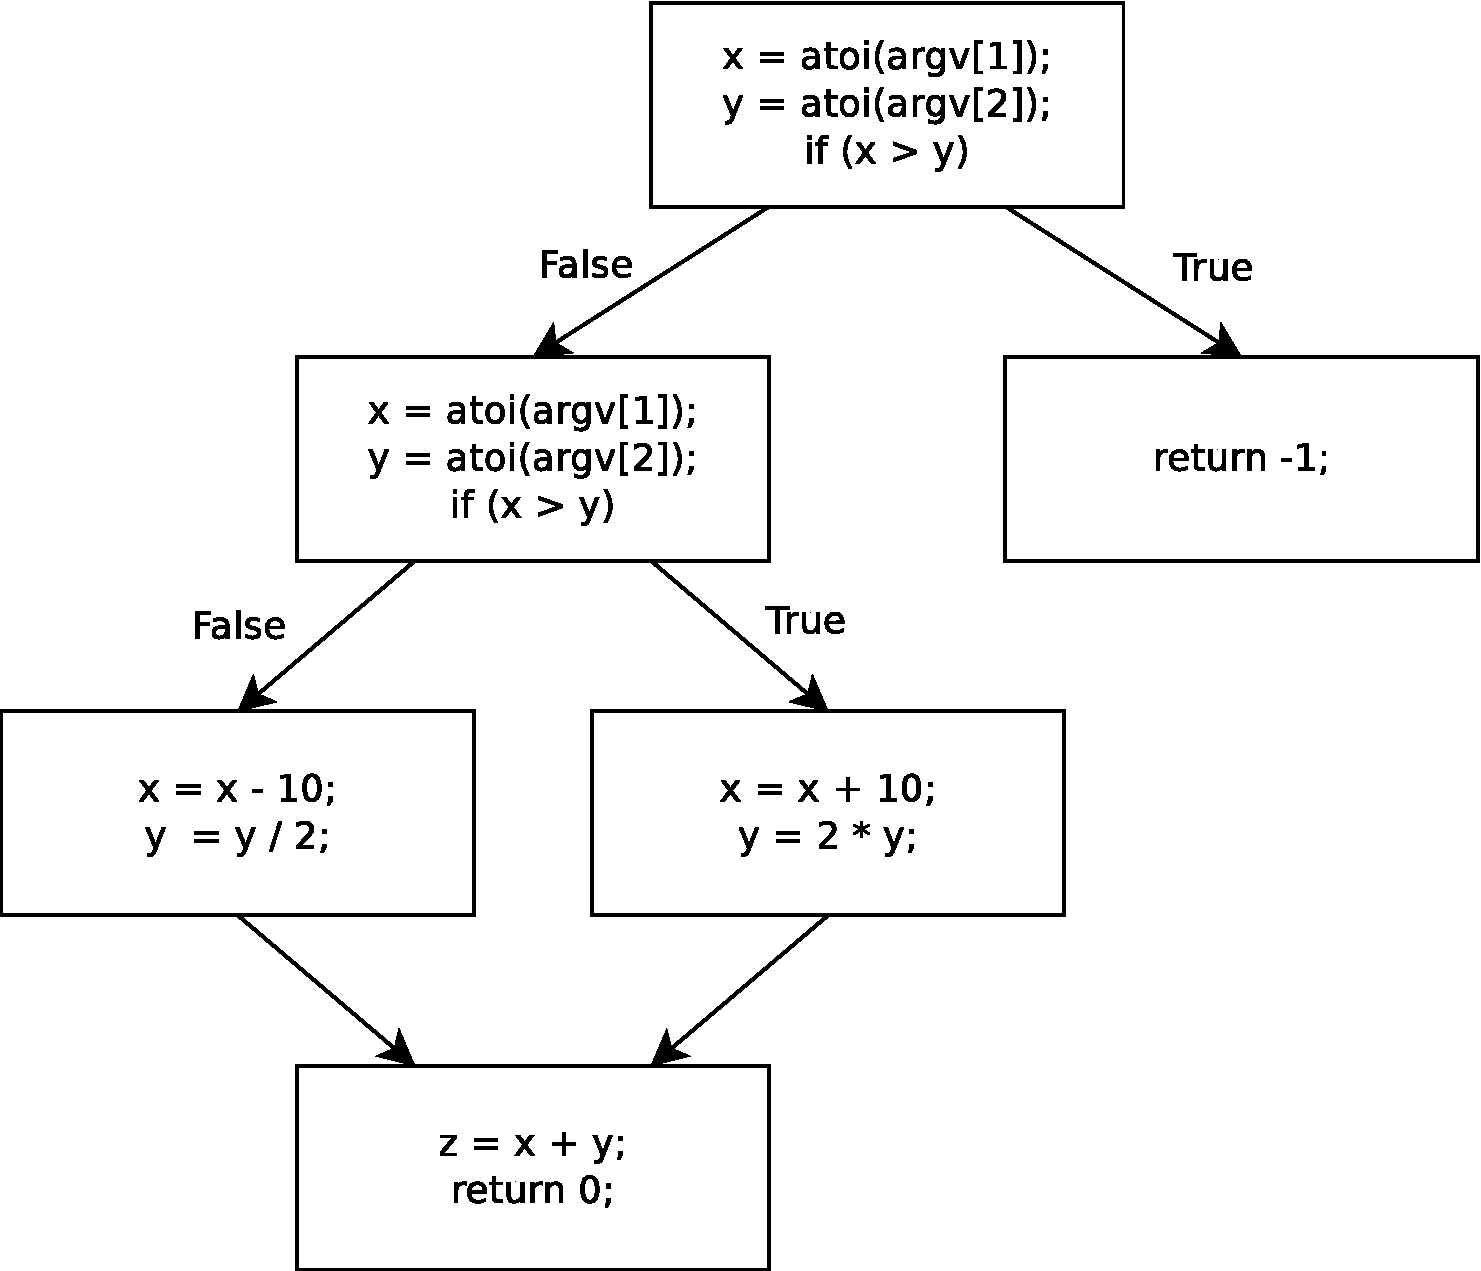
\includegraphics[width=0.6\textwidth]{inc/dia/cfg-example}
  \caption{Пример графа потока управления}
  \label{fig:cfg-example}
\end{figure}

\section{Существующие методы поиска гонок}

Основными методами поиска гонок в программах являются:

\begin{itemize}
  \item формальная верификация,
  \item динамические методы,
  \item статические методы.
\end{itemize}

Формальная верификация основана на установлении соответствия между программой и требованиями к программе, описывающими цель разработки \cite{Kropacheva}. Основными методами, используемыми при формальной верификации, являются метод проверки моделей и дедуктивный анализ.

Основная идея дедуктивного анализа состоит в том, что программа  последовательными преобразованиями приводится в формулу логики. Требования к программе либо изначально формулируются на языке логики, либо переводятся с какого-либо языка на язык логики. После этого доказательство корректности программы сводится к доказательству эквивалентности этих двух формул, что осуществляется с помощью методов, разработанных в логике. Данный метод хорошо разработан для последовательных программ, для параллельных – процесс сильно усложняется \cite{Kropacheva}.

Метод проверки моделей основан на том, что желаемые свойства поведения реагирующей системы проверяются на заданной системе (модели) путём исчерпывающего перебора всех состояний, достижимых системой, и всех поведений (путей), проходящих через эти состояния \cite{Peled}. Основным недостатком данного метода является <<комбинаторный взрыв>> в пространстве состояний, возникающий в случае, когда исследуемая система состоит из многих компонент, переходы в которых выполняются параллельно.

Динамические методы основаны на изучении потока событий, генерируемых программой во время выполнения \cite{Kovega}. Недостатком данных методов является то, что состояние гонки может быть зафиксировано, только если оно возникло в проверяемом  варианте исполнения программы, а, значит, нет гарантии, что оно не может возникнуть в каком-то ином случае. Другим существенным недостатком является то, что большинство средств динамического анализа зависит от оснащения приложения средствами мониторинга, что может менять поведение исполняющей среды.

Статические методы основаны на анализе исходного кода программы. Достоинством данных методов является теоретическая возможность анализа всех возможных путей выполнения программы. Недостатком является наличие большого количества ошибок второго рода,  обнаружения ситуаций гонок в тех местах программы, где их нет, что усложняет анализ и выявление тех результатов, которые соответствуют действительным ситуациям гонок. Примером такой ситуации является инициализация переменных в момент, когда программа выполняется в рамках только одного процесса или потока.

\section{Статические методы поиска гонок}

Основными методами статического поиска гонок являются:

\begin{itemize}
  \item аннотирование кода,
  \item анализ потока выполнения программы.
\end{itemize}

Аннотирование кода выполняется за счёт добавления в исходный код программы специальных конструкций, содержащих информацию об объектах взаимоисключения, обеспечивающих защиту доступа к переменным и вызовам функций. В листинге~\ref{lst:annotated1} и листинге~\ref{lst:annotated2} представлены примеры разных способов аннотирования кода для контроля захвата блокировок при доступе к переменным или функциям. Недостатком данного метода является необходимость добавления большого числа аннотаций, что влечет за собой увеличение объема кода, а, следовательно, и ухудшение его читаемости. Кроме того не исключена возможность допущения ошибок при самом аннотировании. Достоинством данного метода является гарантированная проверка захвата необходимых объектов взаимоисключения, указанных в аннотации, за исключением особых случаев, например, таких, как захват блокировки в условии (условная блокировка) и доступ к элементам массива. Примеры таких случаев продемонстрированы в листинге ~\ref{lst:annotated3}.

\lstinputlisting[language=C,caption=Пример аннотирования кода (\Code{annotated1.java}),label=lst:annotated1]{inc/src/annotated1.java}

\lstinputlisting[language=C,caption=Пример аннотирования кода (\Code{annotated2.cpp}),label=lst:annotated2]{inc/src/annotated2.cpp}

\lstinputlisting[language=C,caption=Пример аннотирования кода (\Code{annotated3.cpp}),label=lst:annotated3]{inc/src/annotated3.cpp}

Анализ потока выполнения программы производится на основе анализа последовательностей выполнения программы с целью выявления параллельно выполняющихся частей программы и переменных, одновременный доступ к которым возможен из нескольких потоков, и блокировок, защищающих доступ к ним.

Основная идея статического поиска гонок заключается в том, чтобы удостовериться, что для каждой общей области памяти существует, по крайней мере, одна блокировка, которая берётся во всех потоках при доступе к этой области. Тогда в случае, когда один поток удерживает блокировку, обеспечивается взаимоисключающий доступ к данным, что позволяет избежать гонок \cite{Vojdani}. Для того, чтобы определить, существует ли общая блокировка, можно вычислить наборы блокировок, которые удерживаются в каждой точке программы. При этом должны отслеживаться только те блокировки, которые захватываются на всех путях, проходящих через рассматриваемую точку. Вычислив множества всегда удерживаемых блокировок для каждой точки программы, достаточно проверить пересечение этих множеств в тех точках, где происходит доступ к исследуемой области памяти. Если пересечение не пусто, то можно сделать вывод о том, что гонки при доступе к данной области памяти отсутствуют, в противном случае существует потенциальная возможность возникновения гонок.

Чтобы применить эти базовые идеи к анализу реальных программ на C, нужно решить некоторые задачи. Прежде всего, нужно определить области памяти, к которым производится доступ, что само по себе является нетривиальной задачей. Даже без динамического выделения памяти нужно провести определение перекрестных ссылок. Например, если два различных указателя, $p$ и $q$, указывают на одну и ту же область памяти, то, например, доступ к полям структуры $p->data$ и $q->data$ может привести к гонкам. Операции захвата и освобождения блокировок на языке C лексически не ограничены, поэтому информацию об указателях необходимо отслеживать с учётом контекста. Рассмотрим пример, представленный листинге~\ref{lst:munge}. Выполнение функции  зависит от контекста, в котором происходит её вызов. В функции последовательно выполняется захват блокировки, увеличение значения переменной и освобождение блокировки. Переменная и блокировка передаются в функцию через указатели. К сожалению, получение информации об указателях с учётом контекста является вычислительно дорогостоящим. Анализ каждого набора значений параметров вызываемой функции на основе полного перебора приводит к комбинаторному взрыву.

\lstinputlisting[language=C,caption=Пример аннотирования кода (\Code{munge.c}),label=lst:munge]{inc/src/munge.c}

Существует три метода статического поиска гонок, позволяющие выполнить анализ кода с учётом контекста выполнения:

\begin{itemize}
  \item Locksmith,
  \item CoBE,
  \item RELAY.
\end{itemize}

Однако контекстная зависимость является не единственной проблемой, возникающей при статическом поиске гонок в программах на языке C. Во-первых, помимо системных мьютексов существуют и другие способы обеспечения монопольного доступа к данным, например, семафоры. Несмотря на то, что поведение семафоров может быть проэмулировано с использованием мьютексов, это может привести к возникновению новых ложных предупреждений. Также при анализе указателей возникают проблемы, связанные с динамическим выделением памяти. И наконец, разрешение проблем, связанных с условными блокировками, также является весьма нетривиальной задачей анализа.

Самым надёжным способом обеспечения отсутствия гонок является исполнение только одного потока. Это связано с тем, что даже в многопоточной программе поток может не всегда выполняться параллельно с другими потоками. Существует много механизмов обеспечения синхронизации без блокировок (англ. lock-free). Например, предположим, что есть главный поток и $n$ рабочих потоков (англ. workers). Главный поток содержит массив $A$ с $n$ элементами (по одному для каждого из потоков) такой, что $A[i]$ влияет на $i$  поток. Более того, предположим, что основной поток инициализирует этот массив перед порождением рабочих потоков (англ. worker threads) и обрабатывает этот массив после завершения всех потоков. Хотя нет блокировок, программа не содержит гонок, т.к. главный поток осуществляет доступ к массиву только тогда, когда рабочие потоки его не имеют; рабочие потоки следуют этому соглашению, что обеспечивает монопольный доступ. Поэтому для решения этой проблемы обычно выделяют временные фазы работы программы такие, как инициализация, обработка и постобработка. Анализатор, имея информацию о том, к каким ресурсам в какие моменты времени производится доступ, должен уметь определять, какие из выполняющихся потоков действительно конфликтуют. Традиционный подход заключается в попытке частично упорядочить инструкции по последовательности исполнения, когда это возможно. Гонка может произойти при одновременном доступе только в том случае, когда нет ограничений последовательности выполнения.

\subsection{Locksmith}

Метод основан на аннотировании программы типами и эффектами. Основной идеей является составление ограничений корреляции между доступами к областям памяти и блокировками. Для каждого доступа к области памяти $p$ c множеством блокировок $L$ составляется ограничение корреляции $p \triangleright L$. Пусть $C$  — множество ограничений, тогда $C \vdash p \triangleright L$ показывает, что ограничение $p \triangleright L$ может быть получено из ограничений в $C$. Множество $S(C, p) = \{L | C \vdash p \triangleright L\}$ обозначает множество всех множест блокировок, которые захватываются при доступе к области $p$. Тогда область памяти $p$ считается защищенной блокировкой при условии, что пересечение всех множеств блокировок является непустым: $\cap S(C, p) \neq \emptyset$. В таком случае говорят, что данные, к которым производится доступ, постоянно коррелируют с множеством блокировок.

В основе данного метода лежит распространение информации об указателях с учётом контекста. Множество обязательно захватываемых блокировок вычисляется с учётом контекста, т.е. с учётом потока выполнения программы. Информация об указателях при этом собирается без учёта контекста (анализируются все присваивания в теле функции независимо от порядка, в котором эти присваивания могут быть выполнены).

Получение множеств блокировок с учётом контекста выполняется на основе анализа потока выполнения программы через граф потока управления. Для этого используются переменные состояния. Они позволяют использовать ограничения реализации (англ. instantiation constraints) для анализа множеств блокировок с учётом контекста и добавляют дополнительную ясность при вызове функций.

Анализ указателей в функции без учёта контекста выполняется за счёт порождения подтипов (англ. sub-typing). Идея состоит в том, что каждая область памяти имеет тип, который ассоциируется меткой области памяти $p$. Вне зависимости от того выполняется ли операция чтения или записи в переменную типа $ref^{p}(\tau)$, порождается ограничение $p \triangleright L$, где $L$ — текущее множество блокировок.

\subsection{CoBE}

Метод состоит из двух этапов. Вначале определяются разделяемые переменные и места, в которых к ним производится доступ. Затем определяются множества удерживаемых блокировок. Если к некоторой разделяемой переменной может осуществляться одновременный доступ из двух различных потоков и множества захваченных блокировок различаются, то возможно возникновение гонок.

Основная идея определения разделяемых переменных состоит в том, что все глобальные переменные и указатели, передаваемые в функции, рассматриваются как разделяемые. Чтобы учесть локальные ссылки на глобальные ресурсы, те указатели, которые используются при непосредственном доступе к данным, а не только служат для передачи адреса, также считаются разделяемыми. Сам по себе анализ указателей основан на идее ускоренного анализа ссылок (англ. Bootstrapping alias analysis) \cite{Bootstrapping}. Его ключевая идея состоит в итеративном проведении процесса анализа таким образом, чтобы с увеличением точности анализа сужался размер анализируемой области (принцип “разделяй и властвуй, распараллеливай и обобщай функции”). Одним из подходящих алгоритмов анализа указателей для инициализации процесса ускоренного анализа  является алгоритм Стинсгарда. Ключевая идея этого алгоритма заключается в том, что в случае, когда указатель $p$ ссылается на две различные области памяти, эти области объединяются, т.е. рассматриваются как единая абстрактная область. В результате получается разбиение указателей на некоторые классы эквивалентности \cite{Steensgaard}. Получив классы эквивалентности, можно применить более точный и дорогостоящий с вычислительной точки зрения алгоритм анализа. Например, в качестве него может быть выбран алгоритм максимально полной последовательности обновлений (англ. Maximally Complete Sequence Update). Он решает задачу анализа указателей следующим образом: два указателя $p$ и $q$ являются эквивалентными, т.е. ссылаются на некоторую общую область $a$, в случае, когда существуют цепочки присваиваний $\pi1$ и $\pi2$, которые семантически эквиваленты присваиваниями $p=a$ и $q=a$.  Для определения эффекта от вызова функции при анализе используется процедура обобщения, которая позволяет вычислить обобщение для функции только один раз и использовать его каждый раз, когда производится вызов этой функции.

Недостатком данного метода является то, что несмотря на то, что анализ указателей производится с учётом контекста в каждой точке программы, различные контексты в которых происходит вызов, не различаются для тела вызываемой функции. Эта проблема решается в следующем описываемом методе — Relay.

\subsection{Relay}

Метод основан на концепции относительного множества блокировок (англ. relative lockset) \cite{Relay}. Эти множества позволяют описать изменения множеств захваченных и освобожденных блокировок относительно точки входа в функцию. Относительные множества блокировок позволяют обобщить поведение функции независимо от контекста её вызова.

При анализе функции обрабатываются изолированно друг от друга снизу вверх в графе вызовов функций. Анализ каждой функции выполняется в 3 этапа:

\begin{itemize}
  \item символьное исполнение,
  \item анализ относительных множеств блокировок,
  \item анализ защищенного доступа.
\end{itemize}

Основа для анализа относительных множеств блокировок и для анализа защищенного доступа закладывается на этапе символьного исполнения программы. Основной задачей этого этапа является выражение значений переменных функции через её формальные параметры и глобальные переменные программы. В ходе анализа для каждой инструкции в программе строится отображение вида $\sum: O->V$, где $O$ и $V$ - множества левых и правых частей операторов присваивания (англ. lvalue и rvalue соответственно), которые используются при символьном исполнении, соответственно. Обозначим через $os \in 2^{o}$ —  множество левых частей оператора присваивания, через $x \in X$  — формальные параметры функции и глобальные переменные программы и через $p \in P$ — узлы представителей классов эквивалентности, полученные с использованием алгоритма Стинсгарда для анализа указателей. Тогда левая часть оператора присваивания $o \in O$  может иметь вид — $x | x.f | p.f | (∗o).f$, а правая — $v \in V$ - $⊥ | T | i | init(o) | must(o) | may(os)$, где $⊥$ означает "значение еще не было присвоено”, $T$ означает "любое возможное значение”, $i$ означает целочисленную константу, $init(o)$  представляет присваиваемое значение, $must(o)$ представляет значение, которое должно указывать на левую часть оператора присваивания $o$, $may(os)$ представляет значение, которое может указывать на любую левую часть операторов присваивания из $os$.

При символьном исполнении функции также следует учитывать влияние, которое могут оказывать другие потоки на состояние переменных. Для определения областей памяти, которые могут быть доступны вне потока, используется алгоритм Стинсгарда. Эти области памяти помечаются символом $T$, означающим, что они могут иметь "любое возможное значение" после каждого вызова функции.

После завершения этапа символьного исполнения, начинается анализ относительных множеств блокировок. Относительным множеством блокировок называется пара $(L_{+}, L_{-})$, состоящая из $L_{+} \in O$ — множества безусловно захватываемых при выполнении блокировок и $L_{-} \in O$ — множества блокировок, которые могут быть освобождены при выполнении. Обозначим множество всех относительных множеств блокировок как $L = 2^{O} \times 2^{O}$. Анализ множества блокировок — это анализ потока данных на решётке $(L, \bot, \top, \sqsubseteq, \sqcup, \sqcap)$, где:
\begin{itemize}
\item $\bot = (O, \emptyset)$, $\top = (\emptyset, O)$
\item $(L_{+}, L_{-}) \sqsubseteq (L_{+}', L_{-}') \Longleftrightarrow L_{+}' \subseteq L_{+} \wedge L_{-} \subseteq L_{-}'$
\item $(L_{+}, L_{-}) \sqcup (L_{+}', L_{-}') = (L_{+} \cap L_{+}', L_{-} \cup L_{-}')$
\item $(L_{+}, L_{-}) \sqcap (L_{+}', L_{-}') = (L_{+} \cup L_{+}', L_{-} \cap L_{-}')$
\end{itemize}

Анализ выполняется снизу вверх в графе вызовов функций. После того, как функция $f$  проанализирована, её влияние на множества блокировок сохраняется как обобщение $LockSummary(f) \in L$, представляющее относительное множество блокировок в конце функции. Обобщение функции $lock(l)$  моделируется относительным множеством блокировок $(\{l\}, \{\})$, а фукнции $unlock(l)$ – $(\{\},\{l\})$. Учитывая вызов функции $e(a)$, для каждой функции $f$, которую может представлять $e$, функция потока сначала получает обобщение $LockSummary(f)$ и затем, используя функцию $rebind$ ($rebind(q, f, e) = q[formal(f ) → eval(e)])$, заменяет все вхождения формальных аргументов функции $f$ на те, которые были переданы фактически. Результирующее обобщение представляет изменения множества блокировок, которое происходит с момента начала выполнения $f$ и до выхода из неё. Чтобы найти относительное множество блокировок после вызова $f$ (в каком-либо месте программы) к нему применяются изменения, задаваемые обобщением $f$.

После окончания анализа множества блокировок для функции выполняется анализ защищенного доступа (англ. guarded access analysis). Под защищенным доступом понимается тройка $a = (o, L, k)$, где $o \in O$ - левые части операторов присваивания, к которым производится доступ, $L \in \mathbf{L}$ – относительное множество блокировок, $k \in K = \{Read, Write\}$ – вид доступа (чтение или запись) в точке доступа. Построение обобщения защищенных доступов для функции аналогично построению обобщения для относительных множеств блокировок за исключением того, что обходить присваивания можно в любом порядке.

На основе данных, полученных после анализа защищённого доступа, производится непосредственное определение мест возможного возникновения гонок. Последовательно просматриваются все возможные пары точек входа в потоки и анализируются их таблицы защищенного доступа. Если в таблицах для двух различных потоков найдется пара строк с одинаковыми значениями левых частей операторов присваивания, и хотя бы в одной из строк указан доступ на запись, такая ситуация свидетельствует о возможном наличии гонки. В результате анализа таблиц появляется большое количество ложных угроз, поэтому необходимо среди всех потенциально опасных операций доступа к памяти выявить те, которые представляют реальную угрозу.

% \section{Методы определения перекрёстных ссылок}
% Бла-бла

\section{Выводы}

Проведен анализ методов поиска гонок в программах. Рассмотрены существующие статические методы поиска гонок в программах на языке Си: Locksmith, CoBE, Relay.
